\documentclass[preprint,12pt]{elsarticle}
\usepackage{amssymb}
\usepackage{lineno}
\usepackage{fixltx2e}
\usepackage{hyperref}
\usepackage{enumitem}
\usepackage{vdmlisting}
\usepackage{float}
\usepackage{pdfpages}
\usepackage{fancyvrb}

\begin{document}

\begin{frontmatter}

\title{Modeling ERTMS/ETCS using VDM++}

%% use optional labels to link authors explicitly to addresses:
%% \author[label1,label2]{<author name>}
%% \address[label1]{<address>}
%% \address[label2]{<address>}

\author{Christian M. Lillelund (201408354)}

\address{School of Engineering, Aarhus University}

\address{Course: E18 - Modeling of Critical Systems}

\begin{abstract}
Modeling of critical systems is an important tool in software engineering, as it allows us to design a system from specification and verify its properties in a unambiguous way early in the development process. In this report, we use the object-oriented Vienna Development Method (VDM++) to model, simulate and verify a subset of the real specifications for the safety-critical European Rail Traffic Management System (ERTMS) standard focusing on those properties of ERTMS that concern interlocking of tracks and safety of the trains. In ERTMS, these features are controlled by the European Train Control System (ETCS) component. With VDM++, we can perform system design analysis and model verification to catch potential faults early before the system is constructed in an implementation language like Java and deployed in a real life context. We start by introducing requirements and invariants based on the ERTMS/ETCS specification and then use VDM++ to design a formal model followed by model-checking. Finally we apply model validation within Overture using VDM++ to verify the correctness of our model and perform a simulation of inputs. The abstract implementation of ERTMS detailed in this report provide a simple but fundamental understanding of the signaling system's behavior and how to describe its constraints.
\end{abstract}

\begin{keyword}
ERTMS \sep ETCS \sep VDM++ \sep Formal methods \sep Interlocking \sep Safety
\end{keyword}

\end{frontmatter}

\section{Introduction}
\label{S:introduction}
The railway domain was identified as a grand challenge of computing science by (\citet{Challenge}) in 2004 because it is understandable by the general public, provides useful features in terms of transportation and pose many concerns for design and controllability. One part of the challenge is improving the feasibility and capacity of modern railway as the world's population is increasing and rail traffic now moves cross borders.

The European Rail Traffic Management System (ERTMS) is a signaling and control standard developed in the start 2000's to address the interoperability issues with cross-border rail traffic in Europe and lack of capacity with legacy systems, as detailed in (\citet{Ghazel2014}). Currently many European countries have their own national stand-alone signaling and control system implemented by a certain set of rules that differ from each country. ERTMS is designed to replace the national systems to make rail transport more frictionless, improve rail capacity and more attractive to consumers. It consists of two primary parts, the European Train Control and Command System (ETCS) to govern the positions and safety of trains, known as the Interlocking (ITL), and the GSM-R radio communications system to send messages between trains and the RadioBlockCenter (RBC). There a three different levels of ERTMS, L1, L2 and L3 detailed by (\citet{Outlook2012}). We consider L2 in this report. L2 introduces the RBC, a Eurobalise that register train movement and omits any track side signaling equipment. When a train computer wants to enter a new route (a set of tracks), it must requests a movement authority (MA) for that section from the RBC, which will see when we explore the model further. ERTMS defines end of authority (EoA) as the point the train is allowed to move to. We consider this aspect as well.

Figure \ref{fig:ertmsoverview} shows the essential components of ERTMS level 2. The train control (EVC) requests movement authorities from the RBC over GSM-R. A typical national railway will have multiple RBC's for each region, where they communicate with a central interlocking service, that receives and tracks the physical location of trains from the Eurobalises in order to either grant or deny movement authority to a train.

\begin{figure}[h]
	\centering
	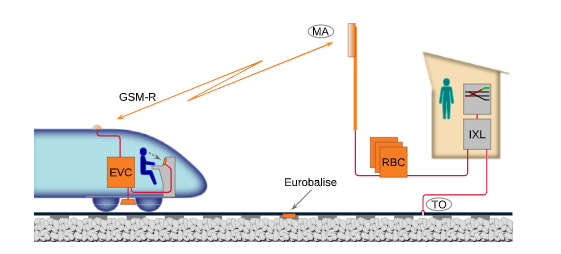
\includegraphics[width=0.8\linewidth]{ERTMS.png}
	\caption{An overview of the ERTMS/ETCS level 2 components. Source: (\citet{Berger2018})}
	\label{fig:ertmsoverview}
\end{figure}

\section{Requirements}
\label{S:requirements}
The purpose of the model is to design and verify the interlocking properties and operating rules of the ETCS system, a part of ERTMS. With the model we aim to show how VDM++ can we used to create and satisfy a subset of the real requirements of ETCS interlocking, abstracting away most of the physical constraints you would have in a real system and focusing on the control mechanisms you find in the RadioBlockCenter and Interlocking components, described in the introduction. Our model should demonstrate a simulated train that interacts with the control system when traversing multiple routes with sets of tracks, as it would in real life, while simultaneously monitoring and adhering to the safety features of the system. We address the following requirements: \\

R1: A train shall not enter a track section which is occupied by another train (same track).\\
R2: A train shall not pass a track boundary without being given a movement authority (MA) to do so.\\
R3: A train shall respect the maximum permitted speed of its current track.\\
R4: Two trains cannot have a MA for the same track at the same time.\\
R5: The system shall not provide an MA for a track that is occupied by a train.\\
R6: The RBC shall not answer MA's for tracks it is not responsible for.\\
R7: The Eurobalise shall report train movement to the Interlocking.\\

The requirements and the behavior of the ETCS control architecture, that we elaborate on in section \ref{S:systemarch}, are inspired from literature (\citet{Berger2018}) and (\citet{Ghazel2014}), that describe, model and verify many of the real functional properties of ERTMS. In this report we choose a portion of these to model and test our requirements \textit{R1-R7}. From the specification of ERTMS one can define a typical usage scenario for a train that wishes to enter a route. Given a train \textit{T1}, a route \textit{Rt} with tracks \textit{Tr\_{1}} from a set of tracks (i=1,..,n), an \textit{RBC} responsible for tracks \textit{TR\textsubscript{n}}, a eurobalise \textit{Eb} mounted on the track that registers physical movement and a central interlocking service \textit{ITL}:

\begin{itemize}[noitemsep]
	\item Train \textit{T} wants to start a route \textit{Rt} and enter track \textit{Tr}. \textit{T} requests MA for route \textit{Rt} from RBC.
	\item RBC contacts the ITL to verify the route is available and clear.
	\item RBC grants MA to train \textit{T} for route \textit{Rt}.
	\item \textit{T} enters track \textit{Tr}.
	\item Eb registers movement and informs ITL.
\end{itemize}

This functionality will be further explored in the model architecture and design.

\section{Model architecture}
\label{S:systemarch}

The architecture of the model represents the entire system as entities, later defined in VDM++ as classes, that encapsulate functionality related to the individual entity. We consider the purpose of our model, that is to express and simulate several important aspects of ERMTS/ETCS, and use the primary components of such system as our entities. These can seen in figure \ref{fig:ertmscontrolarchitecture} that show a way to model the control architecture of ERTMS based on the real specification set for ERTMS level 2 detailed in (\citet{Berger2018}), but junction control and route guidance has been omitted.

\begin{figure}[h]
	\centering
	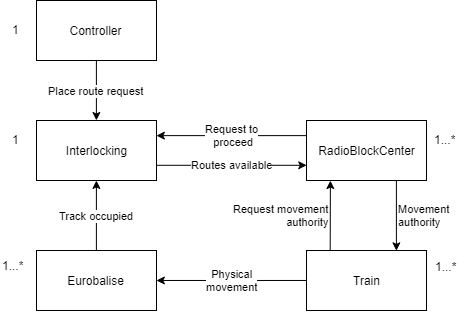
\includegraphics[width=0.8\linewidth]{ERTMSControl.png}
	\caption{The ETCS control architecture partly from the real specification.}
	\label{fig:ertmscontrolarchitecture}
\end{figure}

We shall describe the components in more detail before designing the model. The \textbf{Controller} places route requests into the interlocking at certain time \textit{t} interval to control the flow of traffic and how many routes can be available concurrently in the rail network, a way to limit congestion. A route is simply a set of tracks. \textbf{Interlocking} receives route requests and stores them in a control table containing available routes. It receives track occupation events from physical units along the track side known as eurobalises and uses this information to update the control table with available routes. The \textbf{RadioBlockCenter} receives MA requests from trains and forwards these to the interlocking. RBC's are responsible for multiple tracks, i.e. a block. The \textbf{Train} sends MA requests to the RBC before entering a new track in a route. For each route with one or many tracks (a line segment with a geographic starting and terminal point) the train must request and obtain a MA. This is also stated in the requirements. Each track has a certain speed limit, and the train must never exceed this. The \textbf{Eurobalise} registers physical movement when trains enter and leave tracks and reports this to the interlocking. 

In a real scenario, the eurobalise sends track and speed information to passing trains and the ETCS would monitor this and eventually slow down trains, if they go too fast. We do not consider this part in our model. The ETCS architecture in figure \ref{fig:ertmscontrolarchitecture}, requirements and functionality will be used to create VDM++ classes, functions and invariants in the next section.

\section{Model design}

In this section we will review the VDM++ model in a top-down approach and elaborate on interesting design choices made. The entities in our architecture are now VDM++ classes, types represent information state objects, and events and requests are described with operations and functions. A full UML class diagram can be found in Appendix C.

\subsection{Controller}

The controller controls at what rate new routes are placed into the interlocking. In a real setting, it regulates the flow of trains and adds a detail of security, as new routes that become available (free of trains) are not immediately placed into the interlocking. Before ERTMS, this track state was represented by a signal with a flashing or constant yellow light. Listing \ref{lst:controller} shows the VDM++ class. Operation SendRouteRequest() is executed sequentially, as it picks a random route from a sequence of routes and requests the route at the interlocking.

\begin{vdmsl}[label=lst:controller,caption=State variables and the SendRouteRequest() operation in the Controller.]
	class Controller
	
	instance variables
	private itl : Interlocking;
	private routes : seq of Interlocking`Route;
	
	operations
	public Step:() ==> ()
	Step() == SendRouteRequest();
	
	private SendRouteRequest:() ==> ()
	SendRouteRequest() ==
	if(len routes > 0) then
		(dcl rn : nat := MATH`rand(len routes)+1;
			itl.RequestRoute(routes(rn));
	);
	...
	end Controller
\end{vdmsl}

\subsection{Interlocking}

The interlocking has three main operations defining core functionality, made as such because they change the state of the class. First operation accepts new route requests from the controller for routes $R_{n}$ and place it into its set of available routes, $availableRoutes$, if tracks are not already occupied. We choose a set for these, as they are finite, the order is not important and duplicate elements should not be significant. Sets also support some useful operators shown later. The second operation receive and store information from corresponding eurobalises (track trackers) about the physical movement of trains in a map. We choose a map for these, as they define lookup operators that allow us to assert if a particular track is occupied or not. The $trackTable$ maps tracks with a given coordinate to either a true or false value, if the track is occupied or not. Third operation respond to the RadionBlockCenter requesting a MA (Movement Authority) on the behalf of trains. We start be defining the implemented types and instance variables shown in listing \ref{lst:itl1}.

Notice the atomic use in the constructor to defer invariant assertion after the assignment.

\begin{vdmsl}[label=lst:itl1,caption=Types and state information and constructor for the Interlocking class.]
	class Interlocking
	...
	types
	public Order = <PROCEED_GRANTED> | <PROCEED_DENIED>;
	public ProceedReply :: message : Order
	routesAvaliable : set of Route;						 
	public Track :: startX : nat
					startY : nat
					endX : nat
					endY : nat
					description : seq of char
					maxSpeed : nat;
	public Route = set of Track;
	instance variables
	private trackTable : map Track to bool;
	private availableRoutes : set of Route;
	inv InvNoDuplicateTrack(availableRoutes);
	inv InvNoTrackAvailableAndOccupied(trackTable,
	 availableRoutes);
	
	public Interlocking: set of Route ==> Interlocking
	Interlocking(rts) ==
	atomic (
		availableRoutes := rts;
		trackTable := { tr |-> false |
			 tr in set GetTracksInRoutes(rts)};
	);
	end Interlocking
\end{vdmsl}

The interlocking has two invariants, $InvNoTrackAvailableAndOccupied$ that makes sure occupied tracks in $trackTable$ and the set of available routes $availableRoutes$ are mutually exclusive, and $InvNoDuplicateTrack$ that makes sure no duplicate track (with the same start and end coordinates) exists in the set of available routes (listing \ref{lst:itl2})

\begin{vdmsl}[label=lst:itl2,caption=Two invariants that check the integrity of available routes and checks for duplicates.]
	public InvNoTrackAvailableAndOccupied: map Track to bool
	 * set of Route -> bool
	InvNoTrackAvailableAndOccupied(trmap, rts) ==
	forall rt in set rts & forall tr in set rt
		& tr not in set dom trmap or trmap(tr) = false;
		
	public InvNoDuplicateTrack: set of Route -> bool
	InvNoDuplicateTrack(srt) ==
	forall rt1 in set srt &
		forall tr1,tr2 in set rt1 & tr1 <> tr2
		=> tr1.startX <> tr2.startX or tr1.endX <> tr2.endX 
		or tr1.startY <> tr2.startY or tr1.endY <> tr2.endY;	
\end{vdmsl}

Next is the $RequestRoute()$ operation called by the controller (listing \ref{lst:itl3}). If the route $rt$ is not in available routes and its tracks are not occupied, we add it to $availableRoutes$ and clear the track.

\begin{vdmsl}[label=lst:itl3,caption=Definition of the SendRouteReques() operation.]
	public RequestRoute: (Route) ==> ()
	RequestRoute(rt) ==
	if (rt not in set availableRoutes and
		forall tr in set rt & tr not in set dom trackTable
		 or trackTable(tr) = false)
		 then (
			availableRoutes := availableRoutes union {rt};
			trackTable := trackTable ++ { tr |-> false |
		 				  tr in set GetTracksInRoutes({rt})};	
		 ) else skip;
	pre card GetTracksInRoute(rt) > 0;	
\end{vdmsl}

$GetTracksInRoute()$ and $GetTracksInRoutes()$ (listing \ref{lst:itl4}) are utility functions that return the tracks in a route or routes using set comprehensions.

\begin{vdmsl}[label=lst:itl4,caption=Definition of two functions that return the tracks.]
	public GetTracksInRoute: Route -> set of Track
	GetTracksInRoute(rt) ==
		{tr | tr in set rt};

	public GetTracksInRoutes: set of Route -> set of Track
	GetTracksInRoutes(rts) ==
		dunion {tr | tr in set {rt | rt in set rts}};
\end{vdmsl}

The next operation $SetTrackState()$ is called by the Eurobalise when a train enters a new track $tr$ or leaves a track. This is passed as an argument by the Eurobalise. We set the track as occupied on enter and remove the routes that intersects with the occupied track from $availableRoutes$. On leave, the track is cleared in the $trackTable$ (listing \ref{lst:itl5}). A precondition states that the track must be known in the track table.

\begin{vdmsl}[label=lst:itl5,caption=Definition of the SetTrackState() operation.]
	public SetTrackState: Track * Eurobalise`TrainState ==> ()
	SetTrackState(tr, sta) ==
	if(sta = <TRAIN_ENTER>) then (
		atomic (
		trackTable := trackTable ++ {tr |-> true};
		availableRoutes := {rts | rts in set availableRoutes
			& rts inter {tr} = {}};
		);
	) else if (sta = <TRAIN_LEAVE>) then
		trackTable := trackTable ++ {tr |-> false}
	pre tr in set dom trackTable;
\end{vdmsl}

Finally the $RequestToProceed()$ operation called by the RadionBlockCenter (listing \ref{lst:itl6}). It returns a proceed granted if the route $ptr$ is in $availableRoutes$ and for all tracks in route $ptr$ none are in the $trackTable$ as occupied. Before a proceed is granted, it removes the route $prt$ from the list of available routes as well all other routes that may contain the same track as $ptr$. Functions $ProceedGranted()$ and $ProceedDenied()$ return the available routes that intersects with the responsible tracks of the RadioBlockCenter.

\begin{vdmsl}[label=lst:itl6,caption=Definition of the RequestToProceed() operation.]
	public RequestToProceed: Route * set of Track ==> ProceedReply
	RequestToProceed(prt, respTrs) ==
	if (card availableRoutes > 0) then (
		if(exists rt in set availableRoutes
		& prt subset rt and forall tr in set prt
		& tr in set dom trackTable) then
			if(forall tr in set prt & trackTable(tr) = false) then (
				availableRoutes := {rts | rts in set availableRoutes
				& forall ptrs in set {prt} & rts inter ptrs = {}};
				return ProceedGranted(respTrs);
			)
			else return ProceedDenied(respTrs)
		else return ProceedDenied(respTrs)
	) else ( return ProceedDenied(respTrs) )
	pre card prt > 0 and card GetTracksInRoutes({prt}) > 0;
\end{vdmsl}

\subsection{RadioBlockCenter}

The RadioBlockCenter receives MA requests from trains and forwards these to the interlocking, basically acting as a gateway but with its own state of available routes and responsible tracks initialized in the constructor. Similar to the interlocking, we use sets here as the order is unimportant and duplicate elements should not count in the model. Also at no point do we need to select certain elements, but operators like membership, intersection and union are important to us. Listing \ref{lst:rbc1} shows the declarations for the RadioBlockCenter.

\begin{vdmsl}[label=lst:rbc1,caption=Definition of class state and constructor for RadioBlockCenter.]
	class RadioBlockCenter
	types
	public MovementAuthorityReply =
	 <MovementAuthorityGranted> | <MovementAuthorityDenied>;
	
	instance variables
	private respTracks : set of Interlocking`Track;
	private availableRoutes : set of Interlocking`Route := {};
	private itl : Interlocking;
	
	public RadioBlockCenter : set of Interlocking`Track
	* Interlocking ==> RadioBlockCenter
	RadioBlockCenter(trs,pitl) ==
		respTracks := trs;
		itl := pitl;
	);
	...
	end RadioBlockCenter
\end{vdmsl}

To receive the MA's, we define a operation $RequestMovementAuthority()$ that takes a certain route $Rt$, checks that the radio block center is responsible for tracks in $Rt$, then forwards a synchronous proceed request to the interlocking and sends the reply back to the train for route $Rt$. The interlocking replies with all available routes that intersects with the responsible tracks, hence it is passed as a parameter (listing \ref{lst:rbc2})

\begin{vdmsl}[label=lst:rbc2,caption=Definition of the public.]
	RequestMovementAuthority: Interlocking`Route
	 ==> MovementAuthorityReply
	RequestMovementAuthority(rt) ==
	(
	if(rt subset respTracks) then (
		dcl msg : Interlocking`Order;
		def mk_Interlocking`ProceedReply(message,rtr)
			 = itl.RequestToProceed(rt, respTracks)
		in ( msg := message; availableRoutes := rtr; );
			if (msg = <PROCEED_GRANTED>)
				then ( return <MovementAuthorityGranted>; )
			else (
				return <MovementAuthorityDenied>;
			)
		) else return <MovementAuthorityDenied>;
	) pre card Interlocking`GetTracksInRoute(rt) > 0;
\end{vdmsl}

\subsection{Eurobalise}

The Eurobalise is a piece of track side equipment that registers the physical movement of trains, as described previously. The class is straightforward, as it simply defines some track it is situated at and the global interlocking system in listing \ref{lst:eb1}.

\begin{vdmsl}[label=lst:eb1,caption={Types, variables, constructor for the Eurobalise.}]
	class Eurobalise
	types
	public TrainState = <TRAIN_ENTER> | <TRAIN_LEAVE>;

	instance variables
	private itl : Interlocking;
	private track: Interlocking`Track;
	
	public Eurobalise : Interlocking * Interlocking`Track
 	==> Eurobalise
	Eurobalise(pitl, tr) ==
	(
		itl := pitl;
		track := tr;
	);
	end Eurobalise			
\end{vdmsl}

The two operations $Enter()$ and $Leave()$ invoke the interlocking for a track $track$ when a train either enters or leaves it (listing \ref{lst:eb2}. $Enter()$ returns the speed limit of the track to the train.

\begin{vdmsl}[label=lst:eb2,caption={The two operations that trains call to register their movement.}]
	public Enter: () ==> nat1
	Enter() == (
		itl.SetTrackState(track, <TRAIN_ENTER>);
		return track.maxSpeed;
	);
	
	public Leave: () ==> ()
	Leave() == (
		itl.SetTrackState(track, <TRAIN_LEAVE>);
	);	
\end{vdmsl}

\subsection{Train}

The Train is the driver of our model and has a route sequence with routes it must traverse. When starting, it invokes the RadioBlockCenter by sending a MA request for the first route $Rt$ in its route sequence, and if the MA is granted, it will enter the first track $Tr$ in route $Rt$ calling the track's respective Eurobalise from the $transponders$ map, set its current speed to match the track, move onto the end and ultimately leave it by calling the Eurobalise. The train will halt should it not obtain a MA for any $Rt$. In our simulation we follow the movement of trains by printing a log of their X and Y positional coordinates as simulation progresses. The train has a lot of state declarations, so for clarity, here we simply show the sequential $Drive()$ operation in listing \ref{lst:train1}. The full code for Train is found in Appendix A.

\begin{vdmsl}[label=lst:train1,caption={Drive() moves the train along a sequence of routes, requests MA for each route and obeys track speed limits.}]
	private Drive: () ==> ()
	Drive() ==
	(
	if (len routeTable > 0
		and state = <Running> or state = <WaitingForSignal>) then (
		dcl currentRoute : Interlocking`Route := hd routeTable;
		if(rbc.RequestMovementAuthority(currentRoute)
		 = <MovementAuthorityGranted>)
		then (
			for track in GetTracksInRoute(currentRoute) do (
				dcl currentEb : Eurobalise := transponders(track);
				atomic (
					state := <Running>;
					currentSpeed := currentEb.Enter()
				);
				posX := track.endX;
				posY := track.endY;
				currentEb.Leave();
				);
			routeTable := tl routeTable;
		) else (
			currentSpeed := 0;
			state := <WaitingForSignal>;
			)
		) else (
			currentSpeed := 0;
			state := <Finished>;
		)
	);
\end{vdmsl}

\section{Validation}

This section describes some of the validation techniques used to ensure correctness of the model. Unit testing was used to test functional properties of classes, combinatorial testing to check logical assertions of the model and lastly proof obligations to find points of interest in the model where state is changed and where these has to guarantee some invariant or logical expression holds.

\subsection{Unit testing}
A typical unit test verifies the functional properties of a class's functions and operations, often conducted in isolation with stubs for any external dependencies. A unit test invokes the unit under test (a class) with some input and evaluates whether the output satisfies what was expected. VDM++ offers unit testing options with VDMUnit, which we have used to test the four control classes in our system and shall explore in a bit. Additionally VDM++ provides a framework for combinatorial testing used to verify pre, post and invariant conditions in our classes. Both methodologies have been applied in this project and the complete set of sets can be found in the attached code, see Appendix A.

\subsection{Combinatorial testing}
The combinatorial tests are defined in the classes as traces and can be seen to the full extend in Appendix A. With these tests we verify preconditions, postconditions and state invariants. As opposed to the unit tests, that fail if any of these are violated, the combinatorial tests print inconclusive in such cases and succeeds no matter the assertion was true or false. Looking at the interlocking, listing \ref{lst:itlcomb1} defines four combinatorial tests that check our invariants. All tests can be seen in Appendix A.

\begin{vdmsl}[label=lst:itlcomb1,caption={Four combinatorial tests that exercise our invariant functions in the Interlocking class.}]
	T1: let trmap in set
	 {{mk_Track(10,5,15,5,"AB",100) |-> false}} in
	InvNoTrackAvailableAndOccupied(trmap, routes);
	
	T2: let trmap in set
	 {{mk_Track(10,5,15,5,"AB",100) |-> true}} in
	InvNoTrackAvailableAndOccupied(trmap, routes);
	
	T3: let rts in set {{{mk_Track(5,5,10,5,"AB",100),
		mk_Track(2,5,10,5,"BA",100)},
		{mk_Track(20,5,10,5,"AB",100),
		mk_Track(30,5,10,5,"DE",100)}}} in
			InvNoDuplicateTrack(rts);
	
	T4: let rt in set {{mk_Track(10,5,15,5,"AB",100),
			mk_Track(15,5,20,5,"BC",100)},
			{mk_Track(20,5,25,5,"AB",100),
			 mk_Track(25,5,30,5,"DE",100)}} in
	let trmap = {mk_Track(10,5,15,5,"AB",100) |-> false} in
	InvIsTrackOccupied(rt, trmap);
\end{vdmsl}

\subsection{Proof obligations}

Overture can generate proof obligations for VDM++ that can be used after model creation to find points of interest in regards to invariant checks, logical assertions, map applications and type compatibilities. The obligations of the model were evaluated and asserted at each point to either help improve the model (eg. by strengthening a precondition), understand where state variables were changed and applied, or to get an overview of invariant checks. Below are three examples from our proof obligation review:

\begin{itemize}
	\item 1. Interlocking-L40: State invariant holds.
	\item 2. Interlocking-L134: Legal map application.
	\item 3. Train-L68: Operation establishes postcondition.
\end{itemize}

The first obligation tells us that the state invariant imposed $availableRoutes$ holds given the assignment of the previously available routes apart from those now reserved in the route request. The second state that the map application done in $InvIsTrackOccupied()$ is legal as the index exists in the domain set of the map. The third states that the operation $AddRoute()$ upholds its postcondition by adding the route to its sequence.

\section{Simulation}

To simulate trains interacting with the control system, we create a $World$ class with two trains running different routes, but sharing a mutual one over a bridge, which they cannot pass at the same time. The World class creates objects for all parts of the environment needed and performs a sequential looping, where we advance the trains and the controller by calling a operation $Step()$. Initially the trains do not have a route set, so we construct our routes based on tracks and use the VDMIO library to print log reports of train movement to the console. Figure \ref{fig:testtrack} shows the track terrain with colors indicating routes for the trains. Both must traverse the line indicated by their color in order to finish. The ERTMS icons show boundaries between tracks. The $World$ class is detailed in Appendix A. The output of the simulation can be viewed in Appendix B.

\begin{figure}[h]
	\centering
	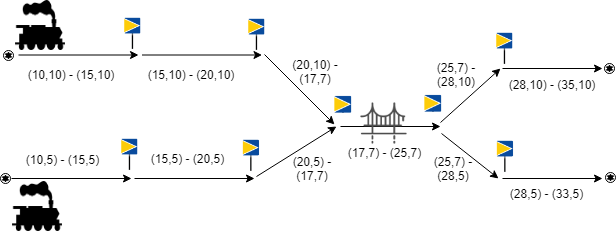
\includegraphics[width=0.8\linewidth]{TrainTrack.png}
	\caption{Two trains on a test track used in the simulation. One follows the green-orange-green route, another the blue-orange-blue route.}
	\label{fig:testtrack}
\end{figure}

\section{Alternatives to the model}

The nature of a real-life ERTMS application is obviously real time, concurrent and multi-threaded. The model of ERTMS level 2 presented in this report is made sequential, that is the execution is performed in steps, as the trains iteratively requests routes to traverse from their route table and cannot move simultaneously, to make it simple for its purpose of conveying the essentials of ERTMS. VDM++ offers a real-time approach to model creation where we define threads as concurrent classes of execution and let our $World$ class implement a $TimeStamp$ class that introduce the notion of time in our model. An obvious benefit of making the model threaded and influenced by time is the transferability to the real-world domain, but introducing this complexity requires us to consider synchronization aspects of threads, shared data and timing constraints. This is a evident next step for this model.

\section{Conclusion}

In this report we have argued why a standardized system like ERTMS and ETCS are indeed needed to cope with interoperability issues presented in current nation-based railway technologies, noted in (\citet{Commission2018}) and why it is suitable for formal modeling. We proceeded to described the architecture behind it and presented a model that all-though simplified, demonstrate the primary entities and interactions in the VDM++ language using Overture. VDM++ constructs were used where appropriate, as we used a set to represent the list of available routes at the Interlocking component, a map to model the physical track table and used a sequence to hold the routes each train has to traverse. We used three techniques Overture offers to validate the correctness of our model and ran a simulation to show the mutual exclusivity of routes and tracks that ETCS impose.

\bibliographystyle{plainnat}
\bibliography{literature}

\appendix
\section*{Appendix A}
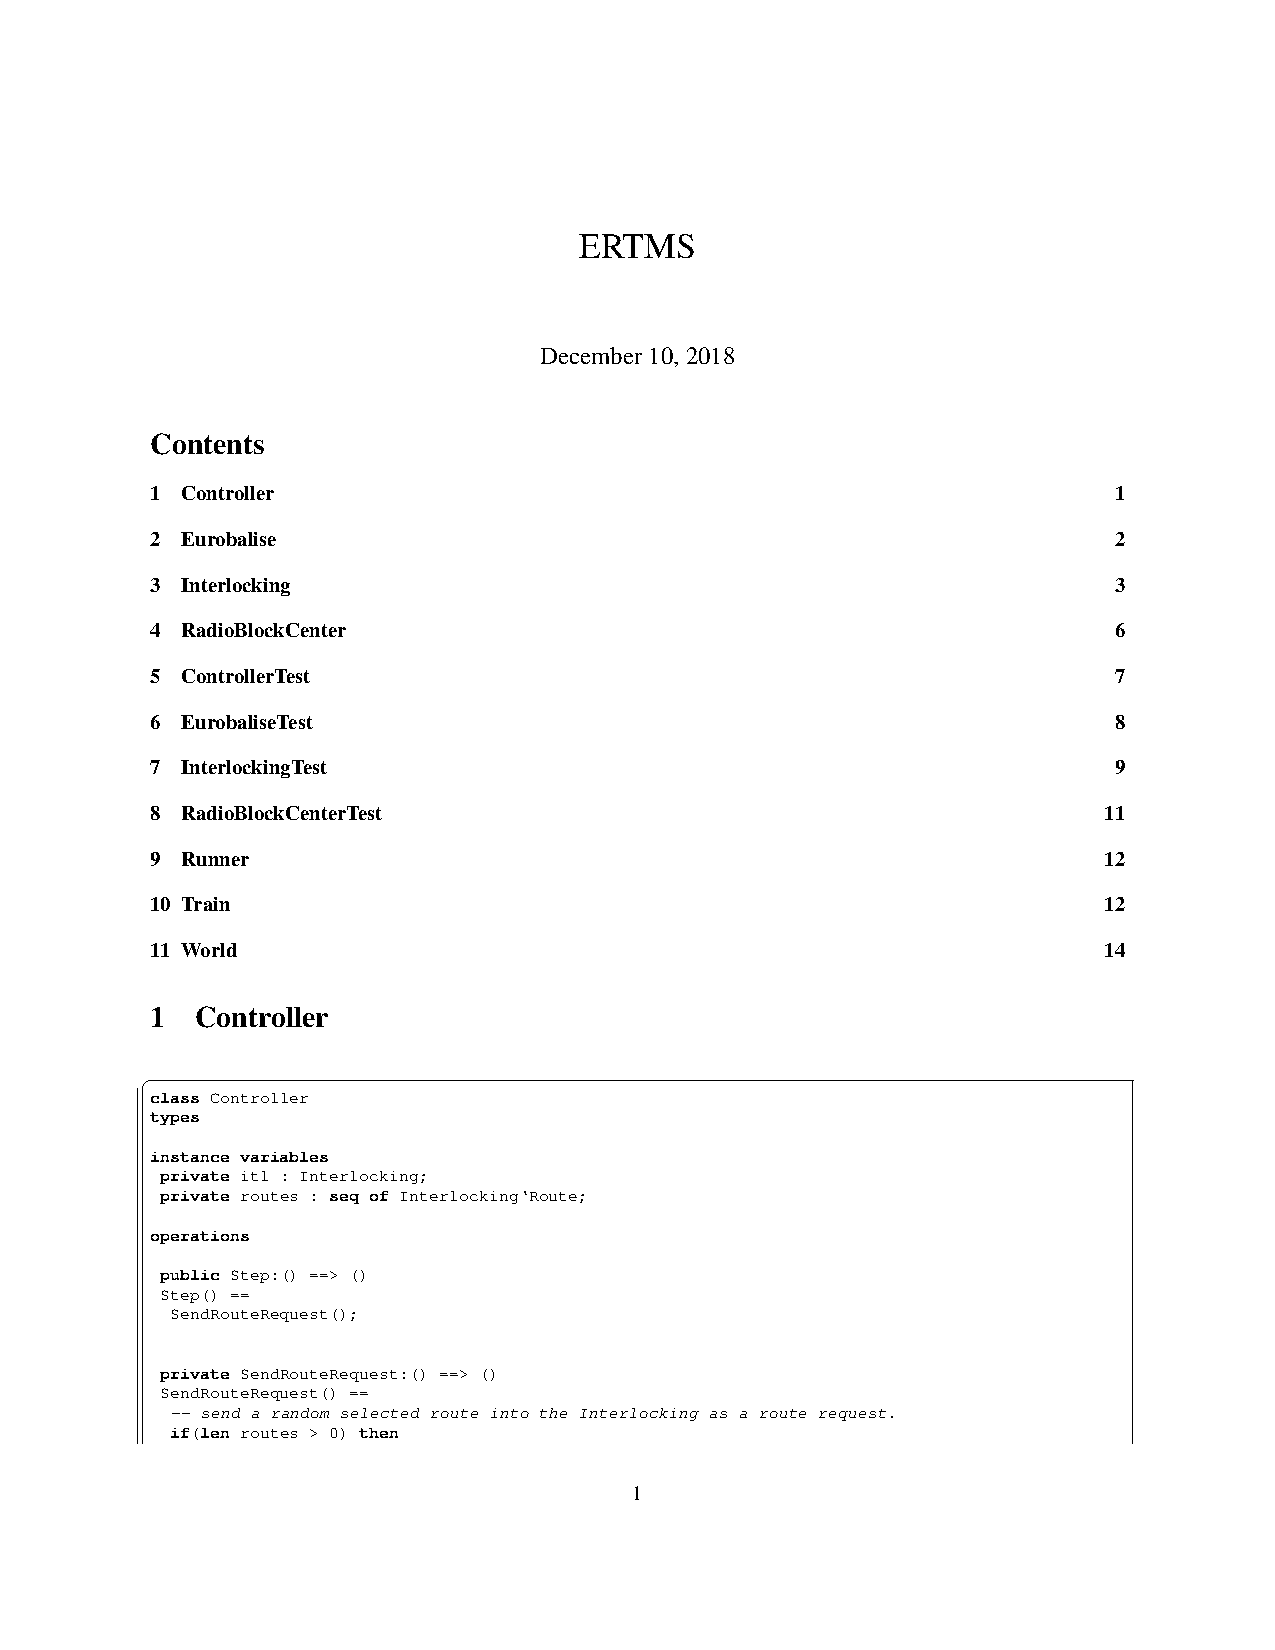
\includepdf[pages=-]{ERTMS.pdf}

\section*{Appendix B}
See attached file SimulationResults.txt.

\section*{Appendix C}
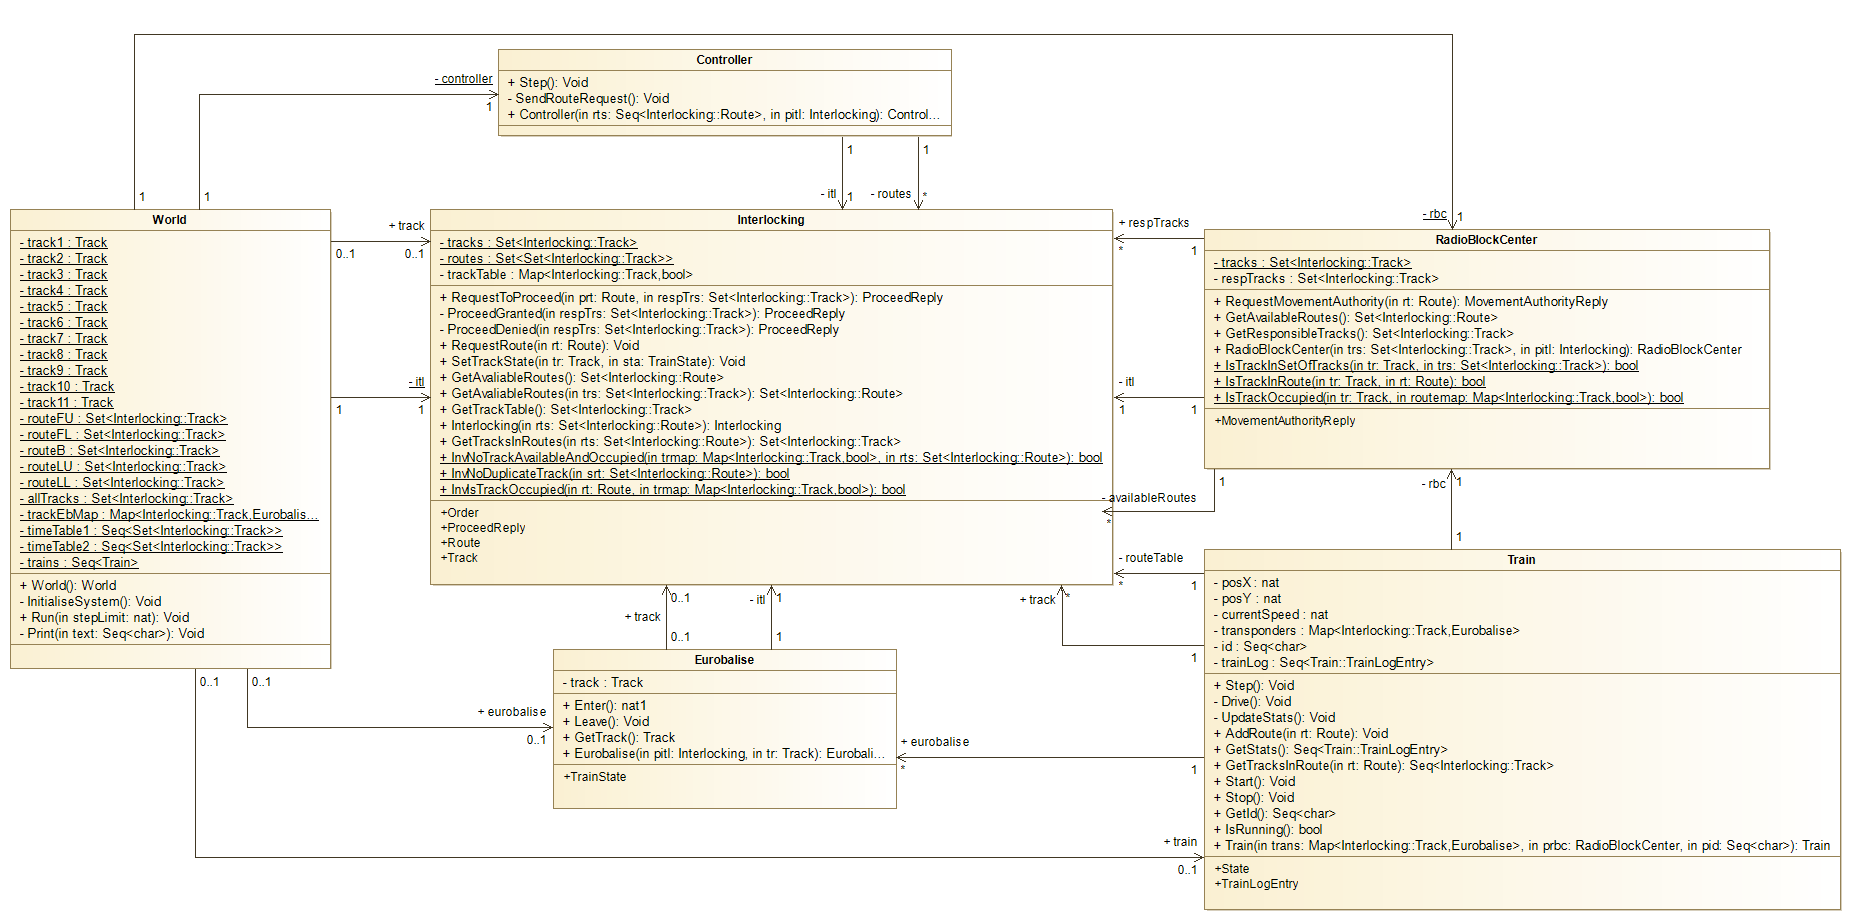
\includegraphics[angle=90,scale=0.35]{ERTMSModel.png}

\end{document}
